\documentclass[../../Atom-ogMolekylefysik.tex]{subfiles}
\begin{document}
\section{Finstruktur i atomer}
\subsection{Atomers magnetisering}
Det vi skal se nu er en ret sjov konsekvens af kvantemekanikken, som blandt andet bruges til atomure og måling af hydrogen i rummet (\SI{21}{cm} linjen). For at komme frem til denne konsekvens skal vi dog først lige forbi noget elektromagnetisme. En ladning i bevægelse vil danne en magnetisk felt. Tilsvarende vil en ladning der bevæger sig igennem et elektrisk felt opleve det som et magnetisk felt på formen.
\begin{equation}
    \v{B}=-\frac{1}{c^2}\v{v}\times\v{E}
\end{equation}
Denne kan udledes fra den specielle relativitetsteori hvor elektriske og magnetiske felter er to sider af samme sag. Vi vil dog ikke vise det her, men i stedet benytte det. Hvis du dog skulle have lyst til at lære mere om den, kan der henvises til stort set alle bøger om speciel relativitetsteori, da det er et meget kendt eksempel at vise.\\
Det elektriske felt vi skal se på er det felt som elektronen udsender, og ligesom vi med tyngdekraften har $F_\text{tyngde}=-\pdif{r}{V}$, hvor $V$ er tyngdepotentialet. Vi kan gøre det samme for det elektriske felt hvis vi bruger det elektrostatiske potentiale som jo bare er givet ved $V=\frac{1}{4\pi\epsilon_0}\frac{q_1q_2}{r}$ vi kan så relatere kraften til det elektriske felt ved at bruge Lorentz formel, der er givet ved: $\v F=e\v E$ og vi ser dermed at $\v E=\frac{1}{e}\pdif{r}{V}\frac{\v{r}}{r}$ (minusset fra kraftformlen går ud med minusset fra elektronens ladning). Vi kan så sætte udtrykket for $V$ ind i udtrykket for $E$ hvilket giver:
\begin{equation}
    \v{E}=\frac{1}{e}\frac{\v{r}}{r}\pdif{r}{}\frac{1}{4\pi\epsilon_0}\frac{-e^2}{r}=\frac{e\v{r}}{4\pi\epsilon_0r^3}
\end{equation}
Hvilket vi sætter ind i formlen fra $B$-feltet, som så giver os:
\begin{equation}
    \v{B}=-\frac{1}{c^2}\v{v}\times\v{E}=-\frac{1}{c^2}\frac{e}{4\pi\epsilon_0r^3}\v{v}\times\v{r}
\end{equation}
Vi har så formlen for to krydsprodukter der siger: $\v{a}\times\v{b}=-\v{b}\times\v{a}$
dette gør så vi kommer af med minus tegnet i vores udtryk, og vi bruger så det matematiske trick at vi ganger med 1 på en smart måde, nemlig $1=\frac{m}{m}$, dette gør vi så vi kan få udtrykket til at se ud på følgende måde:
\begin{equation}
    \v{B}=\frac{1}{mc^2}\frac{e}{4\pi\epsilon_0r^3}\v{r}\times m\v{v}
\end{equation}
Vi kan her se at udtrykket $\v{r}\times m\v{v}$ jo er det angulære moment, eller impulsmomentet. hvilket kvantemekanisk har enheder af $m\hbar$ hvor m er kvantetallet der kommer fra løsningen til Schrödingerligningen for hydrogenatomet. Vi kan derfor sige at $\v{r}\times m\v{v}=\hbar\hat{l}$, hvor $\hat{l}$ er den operator der måler projektionen af det angulære moment langs z aksen, hvilket er det samme som m kvantetallet. Dette kan vi indsætte i udtrykket og vi får derfor at det $B$-felt som elektronen laver når den flyver rundt om protonen kan beskrives ved følgende formel:
\begin{equation}
    \v{B}=\frac{\hbar}{mc^2}\frac{e}{4\pi\epsilon_0r^3}\hat{l}
\end{equation}
\subsubsection*{Spin-orbit kobling}
Et godt spørgsmål er så at spørge sig selv om hvorfor vi gjorde alt det her? Grunden er at de energiniveauer vi måler hydrogenatomet til at have, afhænger af hvor stort et magnetfelt, der påvirker elektronen. Det er nemlig sådan at der er en kobling mellem elektronens spin og magnetiske felter, hvilket får energierne til at blive splittet op så de ikke kun afhænger af $E_n$, som jo er løsningen til Schrödingerligningen, men også afhænger af denne kobling mellem spinnet og det angulære moment. Det er sådan at hvis der er en kobling mellem to ting, der påvirker energiniveauet af et system, så opskriver man denne kobling som en Hamiltonoperator og man kalder det også en hamiltonian. For koblingen mellem spinnet og det angulære moment får vi at koblingen er givet som $H_{s-o}=\v{\mu}\cdot\v{B}$ hvor vi kan indsætte vores nyligt fundne værdi for $\v{B}$ og inkludere at $\v{\mu}=g_s\mu_B\hat{s}$, hvor $\hat{s}$ er spinoperatoren.
\begin{equation}
    H_{s-o}=\v{\mu}\cdot\v{B}=g_s\mu_B\hat{s}\frac{\hbar}{mc^2}\frac{e}{4\pi\epsilon_0r^3}\hat{l}=\v{\mu}\cdot\v{B}=g_s\frac{\hbar^2}{2m^2c^2}\frac{e^2}{4\pi\epsilon_0r^3}\hat{s}\cdot\hat{l}
\end{equation}
da Bohr magnetonen $\mu_B$ er givet ved: $\mu_B=\frac{e\hbar}{2m}$.\\
\\
Vi har nu en ny hamiltonian, der beskriver hvordan elektronens bindingsenergi bliver påvirket af det B-felt, som elektronen laver omkring protonen. Måden hvorpå vi inkorporerer det i den Hamiltonian der beskriver bindingsenergien, er simpelthen af vi bare lægger dem sammen, så vi får:
\begin{equation}
    H_{tot}=H_{binding}+H_{s-o}
\end{equation}
Så når vi tager den nye hamiltonian og udregner forventningsværdien af en tilstand får vi:
\begin{align*}
    \left<E\right>&=\left<\psi_{nlm}|H_{tot}|\psi_{n'l'm'}\right>\\
    &=\left<\psi_{nlm}|H_{binding}|\psi_{n'l'm'}\right>+\left<\psi_{nlm}|H_{s-o}|\psi_{n'l'm'}\right>\\
    &=E_{n}+\alpha\left<\psi_{nlm}\right|\frac{\hat{s}\cdot\hat{l}}{r^3}\left|\psi_{n'l'm'}\right>
\end{align*}
Her har vi gjort det smarte at vi har absorberet alle konstanterne ind i $\alpha$, og $\alpha$ er derfor givet ved: $\alpha=\frac{g_s\hbar^2e^2}{2m^2c^24\pi\epsilon_0}$. $\left<E_n\right>$ er så bare de stationære energier vi i forvejen kender. Det vi derfor nu har tilbage er at vi skal finde ud af hvad udtrykket $\left<\psi_{nlm}\right|\frac{\hat{s}\cdot\hat{l}}{r^3}\left|\psi_{n'l'm'}\right>$ bliver. Det svære i dette udtryk er at finde ud af hvordan operatorne $\hat{s}$ og $\hat{l}$, virker på tilstandene $\psi_{nlm}$. Det første, vi skal teste, er om de kommuterer med hamiltonoperatoren for bindingsenergien. Grunden til at vi spørger om dette, er at tilstandene $\psi_{nlm}$ jo er egentilstande for $H_{binding}$, så ved at tjekke om de to operatorer kommuterer med hamiltonoperatoren, kan vi tjekke om de har et komplet sæt af fælles egentilstande, for hvis vi har det, kan vi benytte Schrödingerligningen til at se at når vi bruger en operator, der opererer ind på dens egentilstand, så får vi bare en konstant gange egentilstanden, hvilket vil gøre det en del lettere at finde ud af hvad udtrykket $\left<\psi_{nlm}\right|\frac{\hat{s}\cdot\hat{l}}{r^3}\left|\psi_{n'l'm'}\right>$ bliver.\\
At vise at de to operatorer kommuterer kan være meget interessant og en lærerig øvelse i hvordan man præcis gør det, men det er ret matematisk og der er ikke særlig meget fysik indblandet i det. Vi vil derfor her bare give resultatet, så vi kan komme frem til den interessante fysik i problemet. Kommutatorerne er derfor givet ved:
\begin{align}
    [\hat{l},\hat{H}]&=0 \hspace{1cm}[\hat{l}^2,\hat{H}]=0\\
    [\hat{s},\hat{H}]&=0 \hspace{1cm}[\hat{s}^2,\hat{H}]=0
\end{align}
Hvilket betyder at vores egentilstande $\psi_{nlm}$ også er egentilstande til disse operatorer. Egentilstandene for $\hat{l}$ og $\hat{l}^2$ operatorne kan vi allerede finde, da egenværdierne er givet ved: 
\begin{equation}
   \hat{l}\psi_{nlm}=\hbar m\psi_{nlm} \hspace{1cm}\hat{l}^2\psi_{nlm}=\hbar^2l(l+1)\psi_{nlm} 
\end{equation}
For at beskrive hvad egenværdierne for spinoperatoren $\hat{s}$ er, skal vi først lige have deres egentilstande. Disse kan også udledes andre steder fra, men måden det sker på er egentlig også bare en masse matematik, så det vil vi ikke gøre her, og bare fortælle hvordan de ser ud. Man får dermed at spin egentilsatendene bare bliver $\chi_{sm_s}$ hvor der gælder at $\left<\chi_{sm_s}|\chi_{sm_s}\right>=1$, disse funktioner har to kvantetal nemlig $s$ og $m_s$, og egenværdierne for $\hat{s}$ og $\hat{s}^2$ operatorne er:
\begin{equation}
   \hat{s}\chi_{sm_s}=\hbar m_s\chi_{sm_s} \hspace{1cm}\hat{s}^2\chi_{sm_s}=\hbar^2s(s+1)\chi_{sm_s} 
\end{equation}
Hvilket minder rigtig meget om egenværdierne for de angulære operatorer. Den totale bølgefunktion for en elektron er derfor givet ved:
$\psi_\text{elektron}=\psi_{nlm}\chi_{sm_s}$, og det er egentlig $\psi_\text{elektron}$ vi benytter, når vi udregner $\left<E\right>$. \\
Nu har vi fundet hvordan operatorerne $\hat{s}$ og $\hat{l}$, virker på vores egentilstande, så det vi nu skal til er at finde ud af hvordan den koblede operator $\hat{s}\cdot\hat{l}$ virker. Det vi derfor gør er at definere det totale angulære moment $j=s+l$, som har værdierne $j=|l+s|, |l+s|-1, ... |l-s|$, og for hver $j$ værdi er der $m_j$ værdier, der ligesom med $m_l$ værdierne for tilstanden for hydrogenatomet, har værdierne, $m_{j}=-j, -j+1, ... j$. Så hvis vi har $l=1$ og $s=\frac{1}{2}$, så får vi følgende tilstande, $j=\frac{3}{2}, \frac{1}{2}$ med $m_j$ værdierne, $m_{j=\frac{3}{2}}=\frac{-3}{2}, \frac{-1}{2},\frac{1}{2},\frac{3}{2}$ og $m_{j=\frac{1}{2}}=\frac{-1}{2},\frac{1}{2}$. Hvis vi i stedet havde valgt at opskrive det ved tilstandene $l$ og $s$, så ville vi for vores $l$ kvantetal få $l=1$, og $m_{l=1}=-1, 0, 1$. Dette kan vi kombinere med vores spin kvantetal og få for $s=\frac{1}{2}$, $m_{s=\frac{1}{2}}=\frac{-1}{2}, \frac{1}{2}$, vi ser derfor at vi for hver $m_s$ kvantetal har 3 $m_l$ kvantetal, hvilket i alt giver os 6 tilstande, præcis ligesom med $j$ kvantetallet. De to forskellige måder at beskrive dette på er derfor ækvivalente. Derudover så er $\hat{j}$ operatorens egenværdier også givet ved:
\begin{equation}
    \hat{j}\left|j, m_j, s, l\right>=\hbar m_j\left|j, m_j, s, l\right> \hspace{1cm} \hat{j}^2\left|j, m_j, s, l\right>=\hbar^2 j(j+1)\left|j, m_j, s, l\right>
\end{equation}
og udover at j og $j^2$ er egentilstande til denne tilstand, så er $\hat{s}^2$ og $\hat{l}^2$ tilstandene også egentilstande hvor vi har:
\begin{equation}
    \hat{s}^2\left|j, m_j, s, l\right>=\hbar^2 s(s+1)\left|j, m_j, s, l\right>\hspace{1cm}\hat{l}^2\left|j, m_j, s, l\right>=\hbar^2 l(l+1)\left|j, m_j, s, l\right>
\end{equation}
Okay, nu kan vi endelig komme videre med vores beskrivelse af hvordan operatorerne $\hat{s}\cdot\hat{l}$ virker på vores tilstande. Vi kan nemlig benytte os af vores definition af $\hat{j}$ operatoren der jo siger: $\hat{j}=(\hat{s}+\hat{l})$, så hvis vi tager denne i anden får vi: 
\begin{equation}
    \hat{j}^2=(\hat{s}+\hat{l})^2=\hat{l}^2+\hat{s}^2+2\hat{s}\cdot\hat{l}
\end{equation}
og vi får fra dette at vi kan opskrive $\hat{s}\cdot\hat{l}$ som:
\begin{equation}
    \hat{s}\cdot\hat{l}=\frac{1}{2}\left(\hat{j}^2-\hat{s}^2-\hat{l}^2\right)
\end{equation}
hvilket når vi opererer dem in på vores tilstande giver:
\begin{equation}
    \left<\psi_{nlm}\right|\frac{1}{2}\left(\hat{j}^2-\hat{s}^2-\hat{l}^2\right)\left|\psi_{n'l'm'}\right>=\frac{1}{2}\left(j(j+1)-s(s+1)-l(l+1)\right)\left<\psi_{nlm}|\psi_{n'l'm'}\right>
\end{equation}
Vi ser derfor at operatoren $\hat{s}\cdot\hat{l}$ bare bliver en konstant, som er bestemt af de specifikke j,l og s kvantetal vores tilstand består af. Vi har så bare at det eneste vi mangler at finde ud af hvad giver er: $\left<\psi_{nlm}\right|\frac{1}{r^3}\left|\psi_{n'l'm'}\right>$, dette er egentlig bare noget matematik, så vi vil ikke gå særlig meget igennem det, men i stedet bare skitsere at måden man løser dette er på er at man udfører integralet som dirac notationen beskriver  og så indse at det kun er den radielle del der har indflydelse, da $Y_l^m$ tilstandene jo ikke har noget at gøre med $\frac{1}{r^3}$, og vi får derfor:
\begin{equation}
    \left<\psi_{nlm}\right|\frac{1}{r^3}\left|\psi_{n'l'm'}\right>=\int_{0}^{\infty}(R_n^l)^{*}\frac{1}{r^3}R_n^lr^2dr=\frac{1}{l(l+\frac{1}{2})(l+1)}\left(\frac{Z}{na_0}\right)^3
\end{equation}
Hvor $Z$ er antallet af protoner i kernen (1 for hydrogen, men dette gør det muligt at udregne forventningsværdien af $\frac{1}{r^3}$ for kerner med stor ladning og kun en enkelt elektron), og $a_0$ er den såkaldte Bohr radius defineret som: $a_0=\frac{\hbar^2}{(e^2/4\pi\epsilon_0)m_e }$
Vi kan så samle alle trådene her til sidst og få at energiniveauerne i hydrogenatomet bliver splittet op med følgende værdier:
\begin{align*}
    \left<E\right>=&E_{n}+\frac{g_s\hbar^2e^2}{2m_e^2c^24\pi\epsilon_0}\frac{1}{l(l+\frac{1}{2})(l+1)}\left(\frac{Ze^2m_e}{n\hbar^24\pi\epsilon_0}\right)^3\frac{1}{2}\left(j(j+1)-s(s+1)-l(l+1)\right)\\
    =&E_{n}+
    \frac{g_sZ^3e^8m_e}{c^2n^3\hbar^44^5\pi^4\epsilon_0^4}
    \frac{\left(j(j+1)-s(s+1)-l(l+1)\right)}{l(l+\frac{1}{2})(l+1)}
\end{align*}
Hvilket er spin-orbit koblingen, som alt sammen kommer fra interaktionen mellem spin og angulært moment, givet ved udtrykket $\hat{s}\cdot\hat{l}$, og vi ser at hvis elektronens angulære moment er 0 så bliver korrektionen til vores egenenergier 0. Nedenfor er en visualisering af hvordan tilstandene bliver splittet op, denne opsplitning er i størrelsesordenen $\frac{1}{100}$, af de egentlig energier, så størrelsesforholdet på billedet er ikke helt korrekt. Bogstaverne $S$, $P$, $D$ er desuden navne på de forskellige $L$ værdier, og tallet nede til højre for bogstaverne er $J$ værdien. Tallet foran bogstaverne angiver $n$ værdien. Dette er bare hvordan man har valgt at opskrive de forskellige tilstande, og rummer altså ikke noget nyt fysik. 
\begin{figure}[h]
    \centering
    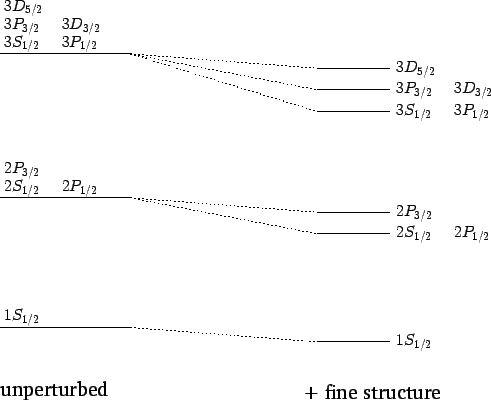
\includegraphics[scale=0.5]{Atom-ogMolekylefysik/billeder/opsplitning.png}
    \caption{opsplitningen af energierne for n=1,2,3 for elektronen i hydrogenatomet}
    \label{fig:amo:vektor-projektion}
\end{figure}
\newpage
\subsubsection*{Generalisering til flere elektroner}
Hvis der er flere elektroner omkring atomkernen kan vi generaliserer udtrykket ovenfor så vi også kan beskrive koblingen mellem spin og angulært moment for disse, dette er relevant hvis man f.eks. vil beskrive Spin-Orbit opsplitningen i Helium eller andre atomer. Vi vil her gøre det for to elektroner, men metoden er valid for generalisering til $N$ elektroner.\\
\\
Hamiltonen for Spin-orbit interaktionen for et par af elektroner er givet ved:
\begin{equation}
    H_{S-O}=\beta_{1}\hat{s}_1\cdot\hat{l}_1+\beta_2\hat{s}_2\cdot\hat{l}_2
\end{equation}
hvor
hvor $\beta_n$ er givet ved:
\begin{equation}
    \beta_n=\frac{g_sZ^3e^8m_e}{c^2n^3\hbar^44^5\pi^4\epsilon_0^4}\frac{1}{l_n(l_n+\frac{1}{2})(l_n+1)}
\end{equation}
hvilket betyder at værdien af $\beta$ afhænger af det angulære moment.\\
I det forrige tilfælde var vi tilfredse med at opstille vores Hamilton på denne måde, fordi l og s ikke ændrede sig, da l jo betegner  det angulære moment, så for at det skal ændre sig skal der komme en udefrakommende kraft der påvirker elektronen. I det tilfælde vi har nu, er det dog sådan at $l_1$ og $l_2$ godt kan ændre sig og give hinanden lidt ekstra angulært moment, hvis de til gengæld mister lidt selv. Dette betyder at $l_1$ og $l_2$ ikke er er bevarede størrelser, men at det totale angulære moment $L=l_1+l_2$ er en bevaret størrelse. For at finde ud af vi kan bruge det til at beskrive vores spin-orbit kobling for flere elektroner skal vi nu til noget der er ret konceptmæssigt svært. Det er nemlig i kvantemekanik sådan at man kan betragte både spin og angulært moment som vektorer. Dette skal ikke forstår som at de er fysiske vektorer man kan sætte ind i et koordinatsystem, men snarere at de kan beskrives i et specielt vektorrum der er en matematisk konstruktion, hvis løsninger giver resultater der passer med eksperimentelle resultater. Denne form for matematisk beskrivelse kaldes gruppeteori og er meget benyttet indenfor blandt andet partikel fysik. Vi vil ikke gennemgå den her, da den er ret matematisk abstrakt og kan være lidt svær at forstå, men vi opfordrer selvfølgelig til at du kigger på det der hjemme hvis det lyder interessant.
Det der dog har en del værdi for os, er at konsekvensen af at $l$ og $s$ kan beskrives som vektorer i det her abstrakte vektorrum, er at normale matematiske regler for hvordan vektorer fungerer også gælder her. Det betyder at vi kan beskrive $l_1$ og $l_2$ ud fra deres projektion ned på store $L$. 
Dette kan klassisk beskrives ud fra følgende formel, hvor man gerne vil projicere vektoren a ned på b.
\begin{equation}
    \v a_b = \frac{\v a\cdot \v b}{|{\v b}|^2}\v b
\end{equation}
\begin{figure}[h]
    \centering
    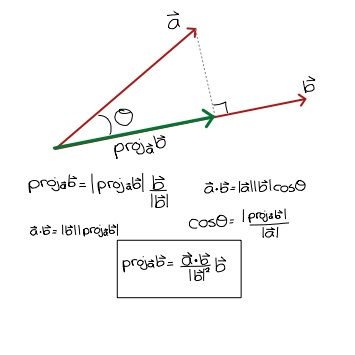
\includegraphics[scale=0.5]{Atom-ogMolekylefysik/billeder/projection.jpg}
    \caption{Projektionen af en vektor a ned på en vektor b}
    \label{fig:amo:vektor-projektion}
\end{figure}\\
Vi kan så ud fra denne formel udlede at projektionen af $l_1$ ned på L må være givet ved:
\begin{equation}
    l_{1,L}=\frac{\left<\hat{l_1}\cdot\hat{L}\right>}{|L|^2}\hat{L}
\end{equation}
Denne formel er vigtig, da projektionen af $l_1$ og $l_2$ ned på L, tilsammen giver L, som man kan se af følgende tegning:
\begin{figure}[h]
    \centering
    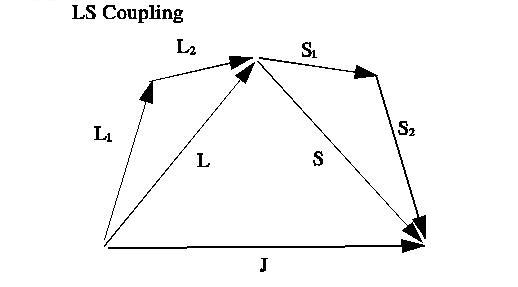
\includegraphics[scale=0.5]{Atom-ogMolekylefysik/billeder/LS-vektor.jpg}
    \caption{${l_1}$ og $l_2$ giver tilsammen L hvis man projicerer dem ned på L}
    \label{fig:amo:vektor-projektion}
\end{figure}\\
Vi ser ud fra billedet at det samme er gældende for spinnet af de to elektroner tilsammen bliver til et totalt spin $S$. Vi kan derfor omskrive vores hamilton $H_{S-O}$ på følgende måde:
\begin{equation}
H_{S-O}=\beta_1\frac{\left<\hat{s_1}\cdot\hat{S}\right>}{\left<\hat{S}^2\right>}\hat{S}\cdot\frac{\left<\hat{l_1}\cdot\hat{L}\right>}{\left<\hat{L}^2\right>}\hat{L}+\beta_2\frac{\left<\hat{s_2}\cdot\hat{S}\right>}{\left<\hat{S}^2\right>}\hat{S}\cdot\frac{\left<\hat{l_2}\cdot\hat{L}\right>}{\left<\hat{L}^2\right>}\hat{L}
\end{equation}
Vi har så at $\left<\hat{L}^2\right>=L(L+1)$ som vi kender det fra tilfældet med en enkelt elektron. Her er forskellen bare at $L=l_1+l_2$ så $L$ har følgende værdier $L=|l_1+l_2|, |l_1+l_2-1|,..,|l_1-l_2|$. så hvis $l_1=l_2=1$ så får L følgende værdier $L=3,1$, hvilket betyder at der kommer mange flere tilstande og at energierne bliver splittet mere op end før. Det fungerer på samme måde med $S=s_1+s_2$, bortset fra at elektroner er fermioner så de har altid spin halv dvs. $s_1=s_2=\frac{1}{2}$. 
Når vi skal udregne $\left<\hat{l_1}\cdot\hat{L}\right>$ så bruger vi at $L=l_1+l_2$ og får:
\begin{align*}
    &\left<\hat{l_1}\cdot\hat{L}\right>\\
    =&\left<\hat{l_1}\cdot(\hat{l_1}+\hat{l_2})\right>\\
    =&\left<\hat{l_1}\cdot\hat{l_1}+\hat{l_1}\cdot\hat{l_2}\right>\\
    =&\left<\hat{l_1}^2+\frac{1}{2}\left(\hat{L}^2-\hat{l_1}^2-\hat{l_2}^2 \right)\right>\\
    =&\frac{1}{2}\left(L(L+1)+l_1(l_1+1)-l_2(l_2+1)\right)
\end{align*}
Læg her mærke til at $l_1$ er positiv inde i parantesen hvis det i stedet er $\left<\hat{l_2}\cdot\hat{L}\right>$ vi vil udregne så vil $l_1$ være negativ og $l_2$ være positiv. Man udregner så $\left<\hat{s_1}\cdot\hat{S}\right>$ og $\left<\hat{s_2}\cdot\hat{S}\right>$ på samme måde. Dette giver så i alt resultatet:
\begin{align*}
    H_{S-O}=\Bigg[&\beta_1\frac{(L(L+1)+l_1(l_1+1)-l_2(l_2+1))(S(S+1)+s_1(s_1+1)-s_2(s_2+1))}{4L(L+1)S(S+1)}\\
    +&\beta_2\frac{(L(L+1)-l_1(l_1+1)+l_2(l_2+1))(S(S+1)-s_1(s_1+1)+s_2(s_2+1))}{4L(L+1)S(S+1)}\Bigg]\hat{S}\cdot\hat{L}
\end{align*}
Herfra går man så over til at beskrive det totale angulære moment som: $\hat{J}=\hat{S}+\hat{L}$ og vi får så ligesom før at $\hat{S}\cdot\hat{L}=\frac{1}{2}\left(\hat{J}^2-\hat{S}^2-\hat{L}^2\right)$ hvor $J$ som sædvanlig har værdierne: $J=|L+S|,|L+S-1|,..,|L-S|$.
Som du kan se bliver det hurtigt totalt uoverskueligt at holde styr på alt dette, og det er derfor man sætter computere til at regne på disse ting hvis man rent faktisk skal udregne hvordan opsplitningen foregår når man har at gøre med flere elektroner, men nu har du set hvordan man rent praktisk skulle gøre det, så hvis du en dag keder dig en stille aften kunne tiden fordrives ved at lave dette i hånden.
\end{document}